\chapter{State of the art}
\textit{This chapter refers to (and summarises) my Master project. Concepts and definitions are essentially inspired by the chapter ten of the book ``Principles of model checking'' \cite{PMC}, the chapter ``Model checking probabilistic systems'' of the course named ``Formal verification of computer systems'' of Mickael Randour \cite{MRV} as well as the article ``Variations on the stochastic shortest path problem'' \cite{DBLP:journals/corr/RandourRS14a}.} \\

Before studying different multi-objective problems in \textit{Markov decision
processes} and defining \textit{strategies} used to solve such problems, we will introduce some fundamental concepts. We will be interested in the cost of \textit{paths} of Markov decision processes as well as the probability to reach some states in these models.
%These measurements cannot be computed without defining a probability measure on events formed with these paths.
To do that, we first need to define a proper \textit{probability measure} on \textit{events} formed with these paths.
So, first of all, we need to define what are \textit{Markov chains}.
Indeed, these stochastic models are essential to define such a probability measure.

\section{Markov chains}
Markov chains are models describing evolutions of stochastic systems.
%The particularity of such systems is that each state inside these models can go to its successors following a probability distribution.
The particularity of such a models is that it evolves from any state to one of its successors following a probability distribution.
%That yields that a Markov chain being in a state and evolving to another one only depends on this state.
That yields that the evolution of a Markov chain, i.e., to go from a state to another one, only depends on the current state of the system.
\begin{definition}[\textbf{Discrete-time Markov chain}]
  A \textit{(weighted) discrete-time Markov chain} (\textbf{MC}) is a stochastic model defined by a tuple $\mathcal{M}=(S, \Delta, w, AP, L)$ where
	\begin{itemize}
		\item $S$ is a countable set of states,
		\item $\Delta: S \times S \rightarrow [0,1] \cap \mathbb{Q}$ is a  \textit{transition function} such that \[\forall s \in S, \sum_{s' \in S}\Delta(s, s')= 1\]
		%\item $d_0:S \rightarrow [0,1]$ est la distribution initiale telle que \[\sum_{s \in S}d_0(s)= 1\] (à noter que dans le cadre de ce document, la distribution initiale peut être omise, et dans ce cas, $\forall s \in S, d_0(s) = \frac{1}{|S|}$).
		where $\Delta(s, s')$ describes the probability that the system goes from state $s$ to state $s'$ in one transition,
    \item $w: S \times S \rightarrow \mathbb{N}_0$ %est la fonction
        %de poids associant à chaque transition un coût strictement positif.
      is a weight function that associates a strictly positive weight to each transition,
    \item $AP$ is a set of atomic propositions, and
    \item $L: S \rightarrow 2^{AP}$ is a labelling function.
	\end{itemize}
\end{definition}
\begin{remark}[\textit{Natural labelling}]
  $AP$ and $L$ are used for \textit{model checking} and can sometimes be omitted. In that case, we consider that $AP = S$ and $L$ is the natural labelling of each state, i.e., for all $s \in S$, $L(s) = \{s\}$.
\end{remark}

\begin{property}
  Let $\mathcal{M} = (S, \Delta, w, AP, L)$ be an MC and $s \in S$ be a state of $\mathcal{M}$. The transition function $\Delta$ defines a probability distribution $\Delta_s: \mathbb{Q} \cap [0, 1], \, s' \mapsto \Delta(s, s')$ on $S$.
\end{property}

\begin{definition}[\textbf{Underlying graph of a Markov chain}]
  Let $\mathcal{M}=(S, \Delta, w, AP, L)$ be an MC. The \textit{underlying graph of} $\mathcal{M}$ is a directed graph $G = (V, E)$ where the states of the MC act as vertices, i.e., $V = S$, and the edges $(s, s') \in E$ of this graph are pair of states $(s, s')\in S^2$ such that $\Delta(s, s')>0$.
\end{definition}

We can represent an MC with its underlying graph, where each edge $(s, s')$ of this graph is labelled with the probability to go from $s$ to $s'$ (i.e., $\Delta(s, s')$) and with the weight of this edge (i.e., $w(s, s')$).
Additionally, labels of each
state can be represented next to it.

\begin{notation}[\textit{Size of an MC}]
  An MC $\mathcal{M}=(S, \Delta, w, AP, L)$ is called \textit{finite} if its state space $S$ is finite. The size of $\mathcal{M}$ corresponds to the number of states of $S$, i.e., $|S|$, plus
the number of edges in the underlying graph of $\mathcal{M}$, i.e., the size of the set
  $\{(s, s') \in S^2 \; | \; \Delta(s, s') > 0 \}$.
\end{notation}

\begin{example}[\textit{Production of solar panels according to weather}]\label{solar-panel}
  Let $\mathcal{M} = (S, \Delta, w, AP, L)$ be the MC of Figure \ref{MCexample}. This system models the production of energy (in $kilo Joules$) of
  an installation of solar panels, according to weather.
  Here, the states are elements of $S = \{s_0, s_1, s_2, s_3\}$ and the atomic propositions are elements of $AP = \{sunny, \, slightly\_cloudy, \, moderately\_cloudy, \, cloudy \}$. The transition function is given by edges in this figure (e.g., $\Delta(s_0, s_1) = \frac{1}{5}$) as well as the
  cost of each transition (e.g., $w(s_0, s_1) = 5$). Finally, labels of states
  are put next to them in orange in the figure (e.g., $L(s_0) = \{sunny\}$).
  \begin{figure}[h!]
    \centering
    \captionsetup{justification=centering}
    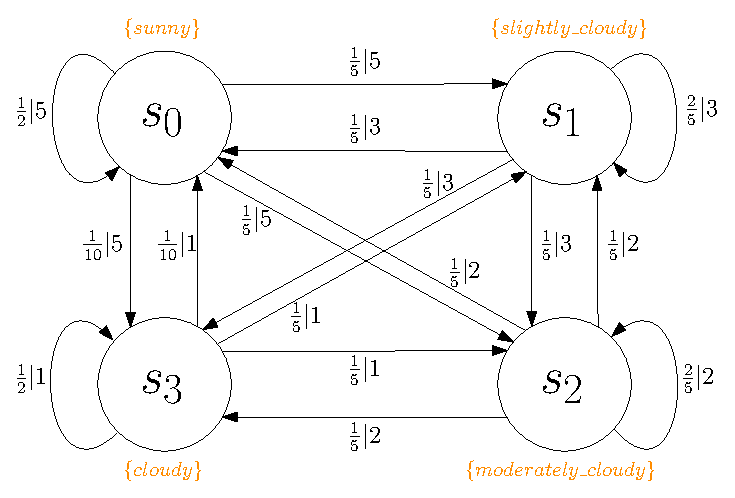
\includegraphics[width=0.6\linewidth]{resources/weather-solar-pannel}
    \caption{MC modelling a daily production of energy (in $kJ$) of solar panels according to weather}
    \label{MCexample}
  \end{figure}
  The way $w$ is defined for this MC yields that, when a day is sunny, the installation produces $5 kJ$ during this day, $3 kJ$ when a day is slightly cloudy, $2 kJ$ when a day is moderately cloudy and, finally, $1 kJ$ when the day is cloudy.
\end{example}

\subsection{Paths of Markov chains}
Before addressing how to compute probabilities in MCs, we must introduce the notion of paths in MCs. Actually, probabilistic events of MCs are sets of paths and prefixes of paths are used to define these events.

\begin{definition}[\textbf{Path of an MC}] Let $\mathcal{M} = (S, \Delta, w, AP, L)$ be an MC.
A \textit{path} $\pi = s_0 s_1 s_2 \dots$ of $\mathcal{M}$ is a (infinite) sequence of states of the MC such that, for all $i \in \mathbb{N}$, $\Delta(s_i, s_{i+1})> 0$. We denote by $Paths(s)$ the set of paths $\pi = s_0s_1s_2\dots$ of $\mathcal{M}$ starting from the state $s \in S$, i.e., such that $s_0 = s$.
\end{definition}
\begin{definition}[\textbf{Finite path of an MC}]
Let $\mathcal{M} = (S, \Delta, w, AP, L)$ be an MC.
A \textbf{finite} path $\hat{\pi} = s_0 \dots s_n$ of $\mathcal{M}$, with $n \in \mathbb{N}$, is a finite sequence of states of $\mathcal{M}$ such that $\Delta(s_i, s_{i+1}) > 0$ for all $i \in \{0, \dots, n-1\}$.
We denote by $Paths_{fin}(s)$ the set of finite paths $\hat{\pi} = s_0 \dots s_n$ starting from the state $s \in S$, i.e., such that $s_0 = s$. Furthermore, all finite paths $\hat{\pi}\in Paths_{fin}(s) = s_0\dots s_n$ is actually a \textit{prefix} of the path
$\pi = s'_0s'_1s'_2 \dots \in Paths(s)$, where $s_i = s'_i$ foral all $i \in \{0, \dots, n\}$. The set of prefixes of the path $\pi$ is denoted by $Prefs(\pi)$.
\end{definition}
% \begin{definition}[\textbf{Prefixes of paths}]
% Let $\mathcal{M} = (S, \Delta, w, AP, L)$ be an MC and $\pi = s_0s_1s_2 \dots$ be a path of $\mathcal{M}$. A prefix of $\pi$ is a finite path $\hat{\pi} = s'_0 \dots s'_n$, with $n \in \mathbb{N}$, such that $s'_i = s_i$ for all $i \in \{0, \dots, n\}$.
% The set of all prefixes of $\pi$ is denoted by $Prefs(\pi)$.
% \end{definition}

\subsection{Probabilities and events in Markov chains}
We will introduce some relevant notions from probability and measure theory.

\begin{definition}[\textbf{$\sigma$-algebra}]
  A $\sigma$-algebra is a pair $(\Omega, \sigma)$ where $\Omega$ is a non-empty set of \textit{outcomes} and $\sigma \in 2^\Omega$ is a set of \textit{events}, complying with the following rules:
  \begin{itemize}
    \item $\emptyset \in \sigma,$
    \item if $E \in \sigma$, then $\overline{E} = \Omega \setminus E$ and $\overline{E} \in \sigma$, and
    \item if $E_i \in \sigma$ for each $i \in \mathbb{N}$, then $\bigcup_{i \in \mathbb{N}} E_i \in \sigma$.
  \end{itemize}
\end{definition}
\begin{definition}[\textbf{Probability measure and space}]
  Let $(\Omega, \sigma)$ be a $\sigma$-algebra. A function $\mathbb{P}: \sigma \rightarrow [0, 1]$ is a \textit{probability measure} on $(\Omega, \sigma)$ and $(\Omega, \sigma, \mathbb{P})$ is a \textit{probability space} iff
  \begin{itemize}
    \item $\mathbb{P}(\Omega) = 1$, and
    \item if $(E_i)_{i \in \mathbb{N}}$ is a disjoint sequence of elements of $\sigma$, then $\mathbb{P}(\bigcup_{i \in \mathbb{N}}E_i) = \sum_{i\in \mathbb{N}}\mathbb{P}(E_i)$.
  \end{itemize}
\end{definition}

We are now interested in probabilistic events of MCs and how measuring them. These events can be formulated with the notion of \textit{cylinder set}.

\begin{definition}[\textbf{Cylinder set}]
Let $\mathcal{M} = (S, \Delta, w, AP, L)$ be an MC, $s \in S$ be a state of $\mathcal{M}$ and $\hat{\pi} \in Paths_{fin}(s)$ be a finite path of $\mathcal{M}$.
\[Cyl(\hat{\pi})=\{\pi\in Paths(s)\;|\;\hat{\pi}\in Prefs(\pi) \} \]
\end{definition}

We can define all events according to this formulation,
with countable union or complementation of cylinder sets. For example, the event consisting of a singleton containing just a single path $\pi = s_0s_1\dots$ is given by $\bigcap_{i \in \mathbb{N}} C_i$, with $C_i = Cyl(s_0s_1\dots s_i)$.

\begin{theorem}[\itshape\bfseries Probability measure]\label{theo1}
  Let $\mathcal{M}=(S, \Delta, w, AP, L)$ be an MC and $s \in S$ be a state of $\mathcal{M}$. There exists an unique probability measure $\mathbb{P}_s$ on the
  $\sigma$-algebra over $Paths(s)$ where the probabilities of cylinder sets are given by
  \[
    \mathbb{P}_s(Cyl(s_0 \dots s_n)) = \prod_{i = 0}^{n - 1} \Delta(s_i, s_{i+1})
  \]
  with $s_0 = s$ and $n \in \mathbb{N}$.
\end{theorem}
\begin{corollary}
Any event defined using complementation or countable union of cylinder sets are also measurable.
\end{corollary}

\begin{example}[\textit{Measuring an event of an MC modelling a solar panel system}]
  Let $\mathcal{M} = (S, \Delta, w, AP, L)$ be the MC of the example \ref{solar-panel}. The probability of sunny weather four days in a row starting on a sunny day is given
  by $\mathbb{P}_{s_0}(Cyl(s_0s_0s_0s_0)) = (\frac{1}{2})^3 = \frac{1}{8}$
\end{example}

\subsection{Reachability in Markov chains} \label{obj-MC}

With this background, we can now introduce some classical problems related to the reachability from a state to a subset of target states in a Markov chain.
We will thus first tackle the reachability problem.
%\subsubsection{Reachability problem}
\begin{definition}[\textbf{Reachability event}]
  Let $\mathcal{M} = (S, \Delta, w, AP, L)$ be an MC and $T \subseteq S$ be a set of target states. The event of reaching $T$, denoted by $\Diamond T$,
  is defined as a countable union of cylinder sets. Indeed, let $s \in S$ be a state of $\mathcal{M}$ and $Paths_{fin}^T(s)$ be the set of finite paths $\hat{\pi} = s_0 \dots s_n \in Paths_{fin}(s)$, such that for all $i \in \{0, \dots, n-1 \}, \, s_i \not \in T$ and $s_n \in T$,
  \[ \Diamond T = \bigcup_{s_0 \dots s_n \in Paths_{fin}^T(s)} Cyl(s_0 \dots s_n) \]
  By definition of $Paths^T_{fin}(s)$, all cylinder sets formed by a prefix from this set are disjoint (all of these prefixes are different, implying disjoint cylinder sets), we can measure $\Diamond T$ with:
  \[
    \mathbb{P}_s(\Diamond T) = \sum_{s_0 \dots s_n \in Paths_{fin}^T(s)}  \mathbb{P}_s(Cyl(s_0 \dots s_n))
  \]
\end{definition}
It remains to compute this probability.

\begin{theorem}[\bfseries\itshape Probabilities of reachability]
Computing $\mathbb{P}_s(\Diamond T)$ for all $s \in S$ can be done in polynomial
time through a system of linear equations (cf. Appendix \ref{app-reach} for more details).
\end{theorem}

% \begin{example}[\textit{Reachability property in an MC modelling a solar panel system}]
%   Let $\mathcal{M}_{sp}$ be the MC modelling the system of the example \ref{solar-panel}.
%    The probability that a cloudy day eventually comes, starting on a sunndy day, is one, i.e., $\mathbb{P}_{s_0}(\Diamond \{s_3\}) = 1$. Indeed, the underlying graph of $\mathcal{M}_{sp}$ is strongly connected, so reaching any state starting from any state has always a probability $1$.
% \end{example}

Now, we will consider the \textit{cost of paths} of an MC. Furthermore, we
are interested in the cost of paths to reach $T$. To compute this cost, we use the \textit{truncated sum function}.

\begin{definition}[\textbf{Truncated sum}]
  Let $\mathcal{M}=(S, \Delta, w, AP, L)$ be an MC, $s \in S$ be a state of $\mathcal{M}$, $\pi = s_0s_1s_2\dots \in Paths(s)$ be a path of $\mathcal{M}$ and $T \subseteq S$ be a set of target states.
  The truncated sum of $\pi$ is the cost to reach $T$ through $\pi$
  for the first time. More formally, the function $TS^T: Paths(s) \rightarrow \mathbb{N} \cup \{\infty\}$ is defined as follows:
	\[
		TS^T(\pi) =
		\begin{cases}
			\sum_{i = 0}^{n-1} w(s_i, s_{i+1}) & \quad \text{if } \forall i \in \{0, \dots, n - 1\}, s_i \not\in T \text{ and } s_n \in T, \\
			\infty & \quad \text{else.}
		\end{cases}
	\]
\end{definition}
With this function, it is now possible to introduce the concept of
expected cost-to-target as well as
the probability of reaching this target set with a bounded cost.

\begin{definition}[\textbf{Expected cost-to-target}]
	Let $\mathcal{M} = (S, \Delta, w, AP, L)$ be an MC, $s \in S$ be a state of $\mathcal{M}$ and $T \subseteq S$ be a set of target states. We define the expected cost to reach $T$, i.e., $\mathbb{E}_s(TS^T)$, corresponding to \textit{the expected truncated sum of paths from $s$ to reach $T$} as follows:
	\begin{itemize}
	\renewcommand{\labelitemi}{\tiny$\bullet$}
	\item If $\mathbb{P}_s(\Diamond T) < 1$, then $\mathbb{E}_s(TS^T) = \infty$.%(par la propriété \ref{prop-ts}).
	\item Else, if $\mathbb{P}_s(\Diamond T) = 1$, then:
	\[
    \mathbb{E}_s(TS^T) = \sum_{c = 0}^\infty c \cdot \mathbb{P}_s(\{\pi \in Paths(s) \; | \; TS^T(\pi) = c \})
  \]
	\end{itemize}
\end{definition}

\begin{remark}[\itshape Infinite expected cost-to-target]
Assume that $\mathbb{P}_s(\Diamond T) < 1$. We enter in the first condition of the definition of $\mathbb{E}_s(TS^T)$, i.e., the expected cost-to-target is infinite. Indeed, let
\[A = \{\pi \in Paths(s) \; | \; \exists \hat{\pi} \in Prefs(\pi), \, \hat{\pi} \in Paths^T_{fin}(s)\}, \text{ and}\]
\[B=\{ \pi \in Paths(s) \; | \; \forall
\hat{\pi} \in Prefs(\pi), \, \pi \not\in Paths^T_{fin}(s)\}.\]
Note that for all $\pi \in B$, $TS^T(\pi) = \infty$ and $A \cup B = Paths(s)$.
As we have assumed that $\mathbb{P}_s(\Diamond T) < 1$
we have $\mathbb{P}_s(B) > 0$, and then
\[
  \mathbb{E}_s(TS^T) = \mathbb{P}_s(A) \cdot \mathbb{E}_s(TS^T | A) + \mathbb{P}_s(B) \cdot \underbrace{\mathbb{E}_s(TS^T | B)}_{=\infty} = \infty.
\]
\end{remark}
\begin{remark}[\textit{Equivalent characterisation of the expected cost-to-target}]
An equivalent characterisation of the expected cost from $s \in S$ to $T$ in case of $\mathbb{P}_s(\Diamond T) = 1$ is given by
\[
  \mathbb{E}_s(TS^T) = \sum_{\hat{\pi} \in Paths_{fin}^T(s)} \mathbb{P}_s(Cyl(\hat{\pi})) \cdot TS^T(\hat{\pi}).
\]
%with $Paths^T_{fin}(s)$, the set of finite paths $\hat{\pi} = s_0 \dots s_n \in Paths_{fin}(s)$  such that, for all $i \in \{0, \dots, n-1\}, s_i \not \in T$ and $s_n \in T$.
Since we can measure the probability of cylinder sets formed by the prefix $\hat{\pi} \in Paths_{fin}^T(s)$ and thanks to these cylinder sets being disjoint, we can compute $\mathbb{E}_s(TS^T)$.
\end{remark}

\begin{theorem}[\bfseries\itshape Solutions of the expected costs-to-target]
  Computing $\mathbb{E}_s(TS^T)$ for all $s \in S$ can be done in polynomial time through a system of linear equations (cf. Appendix \ref{app-expMC} for more details).
\end{theorem}

The last concept that we will define in MCs is the cost-bounded reachability.

\begin{definition}[\textbf{Cost-bounded reachability probability}]
	Let $\mathcal{M} = (S, \Delta, w, AP, L)$ be an MC, $s \in S$ be a state of $\mathcal{M}$, $T \subseteq S$ be a set of target states and $l \in \mathbb{N}$ be a cost threshold.
  The \textit{probability to reach $T$ from $s$ with a cost bounded by the threshold $l$} is defined as follows:
	\[
    \mathbb{P}_s(\Diamond_{\leq l} T) = \mathbb{P}_s(\{\pi \in Paths(s) \; | \; TS^T(\pi) \leq l \})
  \]
\end{definition}
The event $\{\pi \in Paths(s) \; | \; TS^T(\pi) \leq l \}$ is actually measurable: it corresponds to a countable union of cylinder sets formed by prefixes of paths for which the truncated sum is less than or equals $l$.%, i.e., $\{ \pi \in \Diamond T \; | \; TS^T(\pi) \leq l \}$.
\begin{theorem}[\bfseries\itshape Probability of the cost-bounded reachability]
  The probability of the cost bounded reachability to a set of target states $T \subseteq S$ from a state $s \in S$ can be computed in pseudo-polynomial time in the size of $\mathcal{M}$ and $l$, through an unfolding of $\mathcal{M}$ up to the threshold $l$.
\end{theorem}

Intuitively, we unfold $\mathcal{M}$ by recording in each state the cost of the
current path, yielding a new MC $\mathcal{M}'$. The new set of target states $T'$ in $\mathcal{M}'$ is the set of
target states in $\mathcal{M}$ that have a current cost less than or equals $l$ (cf.
Appendix \ref{app-cbrMC} for more details).
Computing the probability of the cost bounded reachability in $\mathcal{M}$ is done by computing the probability of reaching $T'$ in $\mathcal{M}'$.
As computing this probability is done in polynomial time in the size of $\mathcal{M}'$, it is done in pseudo-polynomial time in the size of $\mathcal{M}$ and $l$.
%Finally, it remains to compute the probability to
%reach these new target states in the unfolded MC.
\\

Now, we will study similar problems, but in different systems subject to nondeterminism.

\section{Markov decision processes}
Markov decision processes are systems that model situations describing both non-deterministic and stochastic evolution.
Indeed, in comparison with Markov chains, a Markov decision process requires a decision making to go from a state $s$ to its successors.
Indeed, a nondeterministic choice, named here an \textit{action}, must be done when the system is in state $s$.
When this action is chosen, the system evolves following the probability distribution formed by $s$ and the action chosen.

\begin{definition}[\textbf{Markov decision process}]
	A \textit{Markov decision process}, (\textbf{MDP}) is a tuple $\mathcal{M}  = (S, A, \Delta, w, AP, L)$ where
	\begin{itemize}
		\item $S$ is a countable set of states,
		\item $A$ is a countable set of actions; we denote by $A(s) \in 2^A$  the set of enabled actions when the system is in state $s$ such that, for all $s \in S$,
    $A(s) \neq \emptyset$,
		\item $\Delta: S \times A \times S \rightarrow [0, 1] \cap \mathbb{Q}$ is the probability transition function such that
		\begin{flalign*}
			&\forall s \in S, \; \forall \alpha \in A(s), \; \sum_{s' \in S} \Delta(s, \alpha, s') = 1 \\
			\text{and } &\forall s, s' \in S, \; \forall \alpha \in A \setminus A(s), \; \Delta(s, \alpha, s') = 0
		\end{flalign*}

			where $\Delta(s, \alpha, s')$ defines the probability of going from $s$ to $s'$ in one transition when the action $\alpha \in A(s)$ is chosen,
    \item $w: A \rightarrow \mathbb{N}_0$ %est la fonction
        %de poids associant à chaque transition un coût strictement positif.
      is a weight function that links a strictly positive weight to each action,
    \item $AP$ is a set of atomic propositions, and
    \item $L: S \rightarrow 2^{AP}$ is a labeling function.
	\end{itemize}
\end{definition}
\begin{remark}[\textit{Natural labelling}]
  Again, $AP$ and $L$ can be omitted. In that case, we consider that $AP=S$ and $L$ is the natural labelling of each state, i.e., for all state $s \in S$, $L(s) = \{s\}$.
\end{remark}

\begin{property}
  Let $\mathcal{M} = (S,A, \Delta, w, AP, L)$ be an MDP, $s \in S$ be a state of $\mathcal{M}$ and $\alpha \in A(s)$ be an enabled action of the state $s$. The transition function $\Delta$ defines a probability distribution $\Delta_{s, \alpha}: [0, 1]\cap \mathbb{Q}, \, s' \mapsto \Delta(s, \alpha, s')$ on $S$.
\end{property}
\begin{property}
  An MC is essentially an MDP where, for each state $s$, $|A(s)| = 1$.
\end{property}

We will now introduce some useful notations.

\begin{notation}[\textit{Successors and predecessors}]
  Let $\mathcal{M}=(S, A, \Delta, w, AP, L)$ be an MDP,
  \begin{itemize}
    \item $Succ(s, \alpha) = \{ s' \in S \; | \; \Delta(s, \alpha, s') > 0 \}$
      is the set of $\alpha$-successors of the state $s \in S$ in the MDP, i.e., the set of possible successors of $s$ when the action $\alpha$ is chosen,
    \item $Pred(s) = \{ s' \in S \; | \; \exists \alpha \in A(s'), \, \Delta(s', \alpha, s) > 0 \}$ is the set of predecessors of the state $s \in S$ in the MDP, and
    \item $Succ(s) = \{ s' \in S \; | \; \exists \alpha \in A(s), \, \Delta(s, \alpha, s') > 0 \}$ is the set of successors of the state $s \in S$ in the MDP.
  \end{itemize}
\end{notation}

%The underlying graph of an MDP $\mathcal{M}$ is a directed graph where vertices are states of $\mathcal{M}$ and each edge starting from a state $s$ to one of its successor $s'$ exists if and only if there exists an enabled action $\alpha$
%of $s$ such that $\Delta(s, \alpha, s') > 0$. For the other elements of the tuple defining $\mathcal{M}$, the graph is essentially caracterised the same way as for an MC.
\begin{definition}[\textbf{Underlying graph of a Markov decision process}]
  Let $\mathcal{M}=(S, A, \Delta, w, AP, L)$ be an MDP. The \textit{underlying graph of} $\mathcal{M}$ is a directed graph $G = (V, E)$ where the states of the MDP act as vertices, i.e., $V = S$, and the edges $(s, s') \in E$ of this graph are pair of states $(s, s')\in S^2$ such that there exists an action $\alpha \in A(s)$ where $\Delta(s, \alpha, s')>0$.
\end{definition}

\begin{notation}[\textit{Size of an MDP}]
  An MDP $\mathcal{M}=(S, A, \Delta, w, AP, L)$ is called \textit{finite} if its state space $S$ is finite. The size of $\mathcal{M}$ corresponds to the size
  of the set $\{(s, \alpha, s') \in S \times A \times S \; | \; \Delta(s, \alpha, s') > 0 \}$.
\end{notation}

\begin{example}\label{simple-mdp}
  Let $\mathcal{M} = (S, A, \Delta, w, AP, L)$ be the MDP of the figure \ref{mdp01}. We have that $S = \{s_0, s_1, s_2\}$, $A = \{\alpha, \beta, \gamma\}$ and $AP=\{a, b\}$. If the system is currently in state $s_0$, labeled with $L(s_0) = \{a\}$, the only available action is $\beta$ (because $A(s_0) = \{\beta\}$).
  The cost of choosing $\beta$ is $w(\beta) = 3$.
  Thus, the system evolves following the probability distribution defined by $\Delta_{s_0, \beta}$: it has a probability of $\frac{1}{2}$
  to go to its $\beta$-successor $s_1$ and a same probability to go to its $\beta$-successor $s_2$. Assume that the system evolves to the state $s_2$, with $L(s_2) = \emptyset$. So, in that case, the system has two possible decisions: $\alpha$ or $\gamma$ (because $A(s_2) = \{\alpha, \gamma\}$). If $\alpha$ is chosen, the system returns to $s_2$ with a probability one and a cost of $w(\alpha) = 5$. Else, if $\gamma$ is chosen, the system goes to $s_0$ with a probability one and a cost of $w(\gamma) = 2$.
  \begin{figure}[h!]
    \centering
    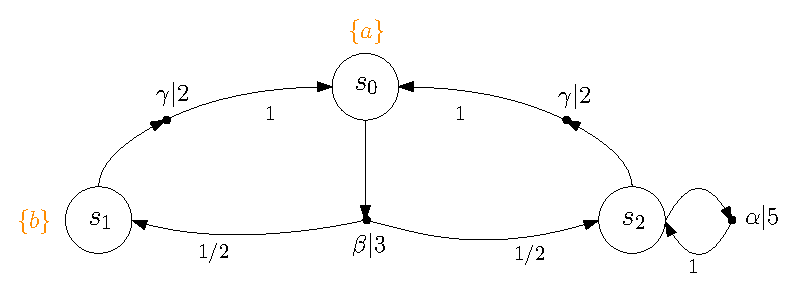
\includegraphics[width=0.7\linewidth]{resources/simple-mdp}
    \caption{MDP with $3$ states, $3$ actions and $2$ atomic propositions}\label{mdp01}
  \end{figure}
\end{example}

\subsection{Strategies in Markov decision processes}
In order to resolve nondeterminism inside MDPs, we need the notions of paths in MDPs and strategies.
\begin{definition}[\textbf{Path in an MDP}]
  Let $\mathcal{M}=(S, A, \Delta, w, AP, L)$ be an MDP and the transition relation
  \[\rightarrow \; =  \{ (s, \alpha, s') \in S \times A \times S \; | \; \Delta(s, \alpha, s') > 0 \}, \,\]
	a path $\pi$ of $\mathcal{M}$ is defined as a sequence of states and actions
	\[ \pi = s_0 \xrightarrow{\alpha_1} s_1 \xrightarrow{\alpha_2} s_2 \xrightarrow{\alpha_3} \dots \]
	Let $s \in S$ be a state of $\mathcal{M}$, we denote by $Paths(s)$ the set of
	paths of $\mathcal{M}$ starting from the state $s$, i.e., such that $s_0 = s$.
\end{definition}
In opposition to MCs, there is no probabilistic space defined on paths of MDPs.
This is related to nondeterminism linked to the choices of possible actions when the system is in a state: when the system enters in a state $s$, an enabled action $\alpha \in A(s)$ must be chosen to allow the system to go to one of its successors according to the probability distribution $\Delta_{s, \alpha}$.
While this action is not chosen, neither probabilistic distribution on the successors of $s$ is defined. That makes this choice purely non-deterministic.
We need strategies to resolve this nondeterminism.
\begin{definition}[\textbf{Histories}]
	Let $\mathcal{M} = (S, A, \Delta, w, AP, L)$ be an MDP. An \textit{history} of $\mathcal{M}$
	is a finite sequence of states $(s_0 \dots s_n) \in S^+$ where for all
	$i \in \{1, \dots, n \} \; \exists \alpha \in A(s_{i-1})$ such that $\Delta(s_{i-1}, \alpha, s_i) > 0$.
	Intuitively, an history is a sequence of states that brought the system from the state $s_0$ to the state $s_n$ along a path of $\mathcal{M}$. The set of histories of $\mathcal{M}$  is given by $\mathcal{H}(\mathcal{M})$.
\end{definition}

\begin{definition}[\textbf{Pure strategy}]
Let $\mathcal{M} = (S, A, \Delta, w, AP, L)$ be an MDP. A \textit{strategy} (also named \textit{policy} or \textit{scheduler} in the literature) for $\mathcal{M}$
	is a function
	$\sigma: \mathcal{H}(\mathcal{M}) \rightarrow A$
	that selects, for a given history $h = (s_0 \dots s_n) \in \mathcal{H}(S)$, an enabled action of $s_n$, i.e., $\sigma(s_0 \dots s_n) = \alpha \in A(s_n)$.
	The path $\pi = s_0 \xrightarrow{\alpha_1} s_1 \xrightarrow{\alpha_2} s_2 \xrightarrow{\alpha_3} \dots$
	is a $\sigma$-path iff $\alpha_i = \sigma(s_0 \dots s_{i-1})$
	for all $i \in \mathbb{N}_0$. The set of $\sigma$-paths starting from the state $s \in S$ is given by $Paths^\sigma(s)$.
\end{definition}
Strategies that we study here are \textit{pure}, i.e., each action is chosen by strategy with probability one. We will see later that \textit{randomised} strategies exist and are essential to resolve some types of problems in MDPs. \\

If a strategy controls the decisions of an MDP, then the nondeterminism is solved
and the MDP acts like an MC. Actually, an MDP $\mathcal{M}$ controlled by a strategy $\sigma$ can be formalised as an MC $\mathcal{M}^\sigma$.

\begin{definition}[\textbf{Markov chain induced by strategy}]
Let $\mathcal{M} = (S, A, \Delta, w, AP, L)$ be an MDP and $\sigma$ be a strategy for
$\mathcal{M}$. The MC induced by $\sigma$ is given by
$ \mathcal{M}^\sigma = (\mathcal{H}(\mathcal{M}), \Delta^\sigma, w^\sigma, AP, L^\sigma) $, where, for all history
$h = s_0 s_1 \dots s_n$ of $\mathcal{M}$,
\begin{itemize}
\item $\Delta^\sigma(h, h . s_{n+1}) = \Delta(s_n, \sigma(h), s_{n+1})$
\item $w^\sigma(h, h . s_{n+1}) = w(\sigma(h))$
\item $L^\sigma(h . s_{n+1}) = L(s_{n+1})$
\end{itemize}
\end{definition}

\begin{property}
  Let $\mathcal{M}$ be an MDP, $\sigma$ be a strategy on $\mathcal{M}$ and $s\in S$ be a state of $\mathcal{M}$. There exists a bijection between the
  set $Paths^\sigma(s)$ on $\mathcal{M}$ and the set $Paths(s)$ on the MC induced by the strategy $\sigma$, $\mathcal{M}^\sigma$.
\end{property}
Since events of an MC are measurable, events of an MDP controlled by a strategy are also measurable through the MC induced by this strategy.
\begin{notation}
  We denote by $\mathbb{P}_s^\sigma$ the probability measure defined on paths starting from the state $s$ of the Markov chain induced by the strategy $\sigma$.
\end{notation}

Markov chains induced by such strategies can be seen as forests of trees representing infinite
unfolding of the MDP where actions are controlled by
strategy (this is due to the fact that the set of histories
of an MDP is infinite). So, such induced MCs have infinite
size. Actually, such strategies are not easy to use in practice because it requires to
know the complete history of the system to decide which action to choose. It is why these strategies have an \textit{infinite-memory}. \textit{Finite-memory strategies} allow to avoid this problem.

\begin{definition}[\textbf{Finite-memory strategy}]
Let $\mathcal{M} = (S, A, \Delta, AP, L)$ be an MDP.
A \textit{finite-memory strategy} $\sigma = (Q, \sigma_\alpha, \delta, \delta_0)$ is a \textit{Moore machine} where
\begin{itemize}
	\item $Q$ is a finite set of \textit{modes},
	\item $\sigma_\alpha: Q \times S \rightarrow A$ is a function that chooses, for any $s \in S$, an action $\alpha \in A(s)$ following a mode $q \in Q$ in which the machine is currently,
	\item $\delta: Q \times S \rightarrow Q$ is the transition function,
	\item $\delta_0: S \rightarrow Q$ is the function that chooses the initial mode of the machine following a state $s \in S$ of the MDP from which the machine is initialised.
\end{itemize}
\end{definition}

\begin{definition}[\textbf{Product of an MDP by a strategy}]
Let $\mathcal{M} = (S, A, \Delta, w, AP, L)$ be an MDP and $\sigma = (Q, \sigma_\alpha, \delta, \delta_0)$ be a finite-memory strategy for $\mathcal{M}$.
The product of $\mathcal{M}$ by $\sigma$ is given by
\[ \mathcal{M} \times \sigma = \mathcal{M}^\sigma = (S \times Q, \Delta^\sigma, w^\sigma, AP, L^\sigma) \]
where $\mathcal{M}^\sigma$ is the MC induced by the finite-memory strategy $\sigma$ and where,
for all states $s, s' \in S$ and for all modes $q, q' \in Q$ of the strategy,
\begin{itemize}
	\item $\Delta^\sigma((s, q), (s', q')) =
	\begin{cases}
	\Delta(s, \sigma_\alpha(q, s), s') & \text{if } \delta(q, s) = q'\\
	0  & \text{else}
	\end{cases}$
  \item $w^\sigma((s, q), (s', q')) = w(\sigma_\alpha(q, s))$
  \item $L^\sigma(s, q) = L(s)$
\end{itemize}
\end{definition}

\begin{example}[\textit{Product of an MDP by a strategy}]
  Let $\mathcal{M}=(S, A, \Delta, w, AP, L)$ be the MDP of the example \ref{simple-mdp} and $\sigma = (Q, \sigma_\alpha, \delta, \delta_0)$ be the
  finite-memory strategy of the figure \ref{finite_mem_strat}.
  \begin{figure}[h!]
    \centering
    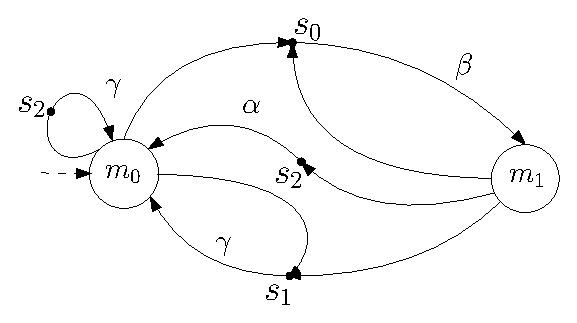
\includegraphics[width=0.4\linewidth]{resources/strategy}
    \caption{finite-memory strategy for $\mathcal{M}$ with $2$ modes}\label{finite_mem_strat}
  \end{figure}

  We assume that, for all $s \in S$, $\delta_0(s) = m_0$. The strategy simply consists in choosing once $\alpha$ when the system enters in the state $s_2$ and choosing $\gamma$ just after that, to return to $s_0$. The MC induced by the product of $\mathcal{M}$ by $\sigma$ is given in the figure
  \ref{inducedMC}.
  \begin{figure}[H]
    \centering
    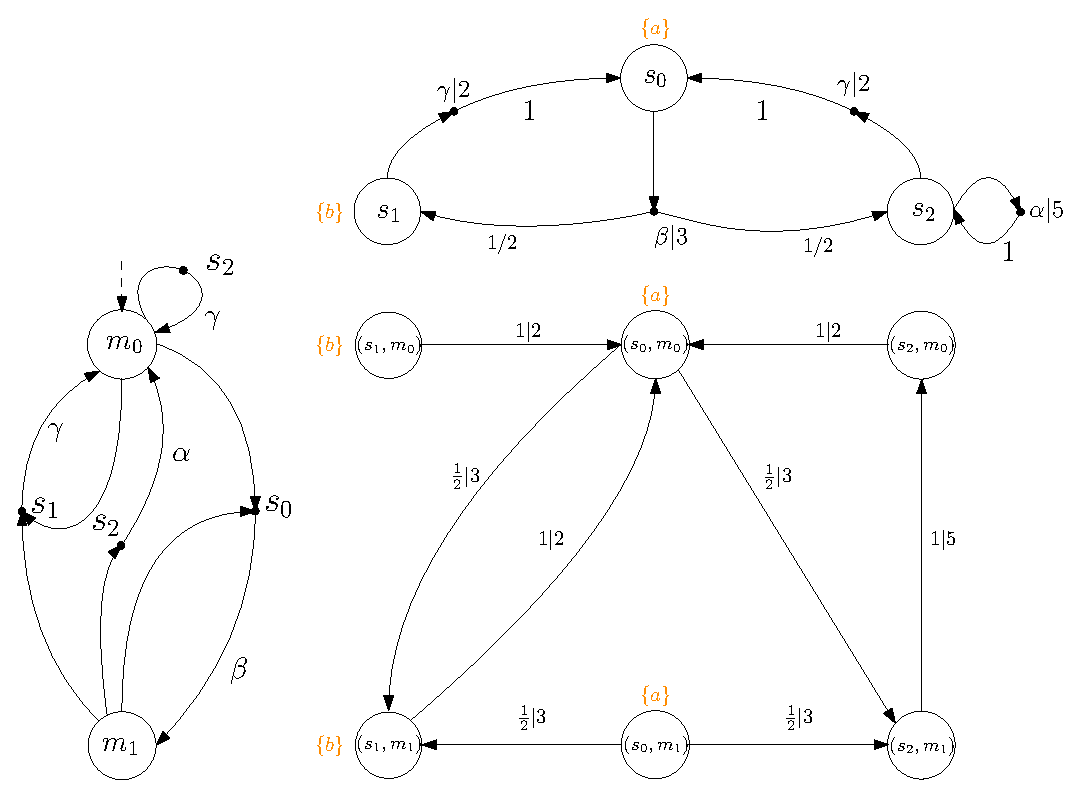
\includegraphics[width=0.55\linewidth]{resources/inductedmarkov}
    \caption{Product of $\mathcal{M}$ by $\sigma$}\label{inducedMC}
  \end{figure}
\end{example}

Finally, the last type of strategy that we will see is a particular case of finite-memory strategies, where strategies have only one mode.
In that case, the action chosen by such a strategy only depends on the current state of the system.

\begin{definition}[\textbf{Memoryless strategy}]
  Let $\mathcal{M}=(S, A, \Delta, w, AP, L)$ be an MDP. A \textit{memoryless strategy} is a function
  $
    \sigma: S \rightarrow A
  $ that links each state $s$ of $\mathcal{M}$ to an enabled action $\alpha \in A(s)$ of this state.
\end{definition}

\subsection{Stochastic problems in Markov decision processes}
Problems that we will address consist in deciding if there exists a winning strategy allowing to verify if properties hold in a MDP.
As for MCs, we will first address the \textit{stochastic reachability problem} in an MDP.
\begin{definition}[\textbf{SR problem}]
  Let $\mathcal{M}=(S, A, \Delta, w, AP, L)$ be an MDP, $s \in S$ be a state of $\mathcal{M}$, $T$ be a set of target states and $\alpha \in [0, 1]$ be
  a probability threshold. The \textit{stochastic reachability} (SR) problem consists
  of deciding if there exists a strategy $\sigma$ such that
  \[
    \mathbb{P}_s^\sigma(\Diamond T) \geq \alpha
  \]
\end{definition}

\begin{theorem}[\bfseries\itshape Solving the SR problem]\label{thm-sr}
  The SR problem can be decided in polynomial time in the size of $\mathcal{M}$
  through a linear program, allowing to build a pure memoryless strategy that gives the optimal actions to reach $T$ from every state $s \in S$ (cf. Appendix \ref{app-sr} for more details).
\end{theorem}

Before introducing the rest, we will first introduce the \textit{truncated sum} of paths of MDPs in order to compute the cost of paths of an MDP.

\begin{definition}[\textbf{Truncated sum for MDPs}]
	Let $\mathcal{M} = (S, A, \Delta, w, AP, L)$ be an MDP, $s \in S$ be a state of $\mathcal{M}$, $T \subseteq S$ be a set of target states and
	$\pi = s_0 \xrightarrow{\alpha_1} s_1 \xrightarrow{\alpha_2} s_2 \xrightarrow{\alpha_3} \dots \in Paths(s)$ be a path of
	$\mathcal{M}$ starting from $s$. The truncated sum $TS^T: Paths(s)
	\rightarrow \mathbb{N} \cup \{\infty\}$ of the path $\pi$ is defined as follows:
	\[
		TS^T(\pi) =
		\begin{cases}
			\sum_{i = 1}^{n} w(\alpha_i) & \quad \text{if } \forall i \in \{0, \dots, n - 1\}, s_i \notin T \text{ and } s_n \in T \\
			\infty & \quad \text{else.}
		\end{cases}
	\]

\end{definition}

By considering the cost of paths of an MDP, we are now interested in building
strategies inducing the shortest path to go from one state to a set of target
states. The notion of shortest path in an MDP is not as obvious as in a graph due to the uncertainty linked to the stochastic environment.
The stochastic shortest path problem in an MDP can be introduced in different
ways. We will first tackle the \textit{stochastic shortest path expectation} problem and
then tackle the \textit{stochastic shortest path percentile} problem. \\

Since events of any MDP controlled by strategy is measurable and
since the cost of paths of any MDP is computable via the truncated sum function, we can
compute the expected length of paths that reach a set of target states using a strategy and, more particularly, build the strategy that will minimise the expected length of these paths.

\begin{definition}[\textbf{SSP-E problem}]
Let $\mathcal{M}=(S, A, \Delta, w, AP, L)$ be an MDP, $s \in S$ be a state of $\mathcal{M}$,
$T \subseteq S$ be a set of target states and $l \in \mathbb{N}$ be a cost threshold. The \textit{stochastic shortest path expectation} (SSP-E) problem
consists in deciding if there exists a strategy $\sigma$ such that
\[
  \mathbb{E}^\sigma_s(TS^T) \leq l
\]
% i.e., if there exists a strategy $\sigma$ such that the expected length of paths starting in the state $s$ in the MC induced by this strategy is lower than the length threshold $l$.
where $\mathbb{E}_s^\sigma(TS^T)$ corresponds to the expected cost of paths starting from $s$ in the MC induced by $\sigma$.
\end{definition}

\begin{theorem}[\bfseries\itshape Solving the SSP-E problem]
  The SSP-E problem can be decided in polynomial time in the size of $\mathcal{M}$, through a linear program, allowing to build a pure memoryless strategy that gives the optimal actions to minimise the expected cost of paths to reach $T$ from every state $s \in S$ (cf. Appendix \ref{app-sspe} for more details).
\end{theorem}

Finally, the last problem that we will present in this chapter is the
\textit{stochastic shortest path percentile} problem. For this problem, we will
be interested to decide if there exists a strategy allowing to reach a set of target states with
a bounded cost with a probability over an high probability threshold.

\begin{definition}[\textbf{SSP-P problem}]
  Let $\mathcal{M} = (S, A, \Delta, w, AP, L)$ be an MDP, $s \in S$ be a state of
  $\mathcal{M}$, $T \subseteq S$ be a set of target states, $l \in \mathbb{N}$
  be a cost threshold and $\alpha \in [0, 1] \cap \mathbb{Q}$ be a probability
  threshold. The \textit{stochastic shortest path percentile} (SSP-P) problem
  consists in deciding if there exists a strategy $\sigma$ such that
  \[
    \mathbb{P}_s^\sigma (\Diamond_{\leq l} T) \geq \alpha
  \]
\end{definition}

\begin{theorem}[\bfseries\itshape Solving the SSP-P problem]
  The SSP-P problem can be decided in pseudo-polynomial time in the size of $\mathcal{M}$ and $l$ by unfolding the MDP $\mathcal{M}$ from the state $s$ up to $l$ and by resolving the SR problem on this unfolded MDP.
  We can build an optimal pure finite-memory strategy in $\mathcal{M}$ that refers to the optimal memoryless strategy satisfying the SR problem in $\mathcal{M'}$.
\end{theorem}

\begin{definition}[\textbf{Unfolded MDP up to a cost threshold}] Let
  $\mathcal{M} = (S, A, \Delta, w, AP, L)$ be an MDP, $s^* \in S$ be a state of
  $\mathcal{M}$, $T \subseteq S$ be a set of target states of $\mathcal{M}$ and $l \in \mathbb{N}$ be a cost threshold.
  Unfolding $\mathcal{M}$ from $s^*$ up to the threshold $l$ can be done as follows: \\
  We build $\mathcal{M}_l = (S_l, A_l, \Delta_l, w, AP, L_l)$ for the subset $T_l \subseteq S_l$ where
  \begin{itemize}
  \item $S_l$ is composed of states $(s, v)$ where $s \in S$ and $v \in \{0, \dots, l\} \cup \{\bot\}$.
  We consider that $\bot > l$, with $\bot + v = \bot$ for all $v \in \{0, \dots, l\}$.
  Intuitively, $v$ records the cost of paths while unfolding $\mathcal{M}$.
  As we unfold $\mathcal{M}$ from $s^*$, we have that
  $(s, 0) \not \in S_l$ for all $s \in S$ such that $s \neq s^*$.
  \item For each $\alpha \in A$, we have that $\alpha \in A_l$ and for all $(s, v) \in S_l$, $A_l(s, v) = A(s)$.
  \item $\Delta_l: S_l \times S_l \rightarrow [0, 1]$ is the probability transition function given by:\\
  $\text{Forall } (s, v), (s', v') \in S_l \text{ and for all } \alpha \in A(s),$
  \[
  \Delta_l((s, v), \alpha, (s', v')) =
  \begin{cases}
  	\Delta(s, \alpha, s') & \quad \quad \text{ if } v' = v + w(\alpha) \leq l \text{ or}\\
  	 & \quad \quad \text{ if } v' = \perp \text{ and } v+w(\alpha) > l \\
  	0 & \quad \quad \text{ else}.
  \end{cases}
  \]
  \item $L_l:S_l \rightarrow AP \mapsto L_l((s, v)) = L(s)$.
  \item Target states are states of
  $T_l = \{(s, v) \;|\; s \in T \wedge v \leq l \}$.
  \end{itemize}
\end{definition}
\begin{remark}[\textit{Optimised unfolding}]
  Since all state $(s, v) \in S_l$ such that $v = \bot$ can never reach $T_l$, it is not useful to keep these states in the unfolded MDP $\mathcal{M}_l$. So, we can replace all these states of $S_l$ with an unique state $s_\bot$ such that, for all $(s, v) \in S_l$ where $v \neq \bot$ and for all $\alpha \in A(s)$ such that $v + w(\alpha) > l$,
  $\Delta_l((s, v), \alpha, s_\bot) = 1$. Then, we define a new action $\alpha_\bot \in A_l$ with an arbitrary weight that will allow a self-loop for $s_\bot$, i.e., $\Delta_l(s_\bot, \alpha_\bot, s_\bot)=1$.
\end{remark}

\begin{example}[\textit{Unfolding of an MDP}]
  Let $\mathcal{M} = (S, A, \Delta, w, AP, L)$ be the MDP of the example \ref{simple-mdp}.
  This MDP can be unfolded from the state $s_0$ up to the threshold $l = 8$ for the target states set $\{s_1\}$ (cf. figure \ref{unfolding}).
  \begin{figure}[h!]
    \centering
    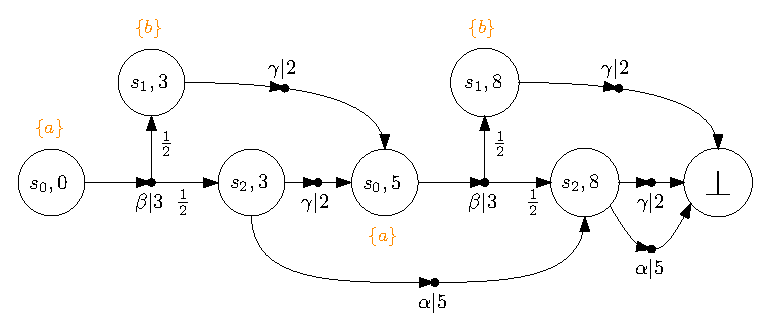
\includegraphics[width=0.8\linewidth]{resources/unfolding}
    \caption{$\mathcal{M}$ unfolded from $s_0$ up to $l=8$ for $\{s_1\}$}\label{unfolding}
  \end{figure}
  The highlighted strategy in the figure \ref{unfolding} is the optimal memoryless strategy satisfying the SR problem in $\mathcal{M}_l$. This strategy is the
  same as the one that resolves the SSP-P problem in $\mathcal{M}$ and is thus finite-memory in $\mathcal{M}$.
\end{example}
